\pagestyle{fancy}
\renewcommand{\theUnit}{8}
\ifthenelse{\isundefined{\UnitPageNumbers}}{}{\setcounter{page}{1}}
\rhead{Chapter  \theUnit: Hypothesis Tests}
\lhead{Math 3382: Statistical Theory}
%\lhead{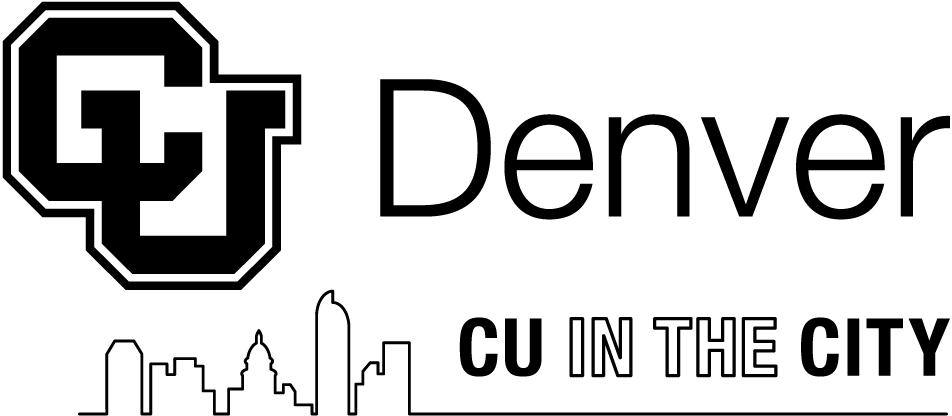
\includegraphics[width=1.25cm]{CUDenver-Logo.png}}
\rfoot{\mypage}
\cfoot{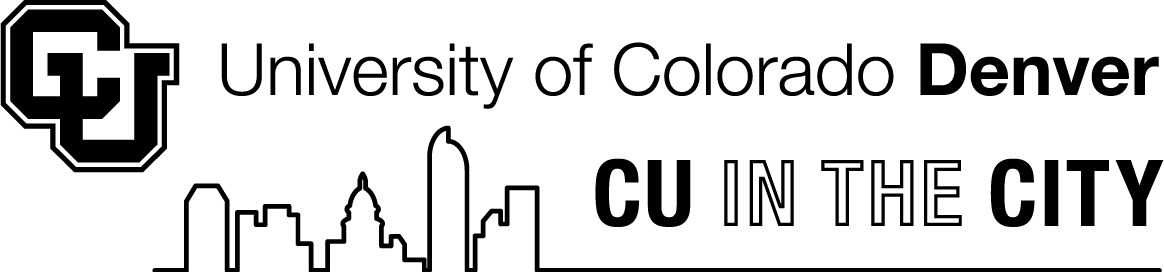
\includegraphics[width=2.25cm]{CUDenver-Logo-coverpage.png}}
\lfoot{Adam Spiegler}
\fancypagestyle{firstfooter}{\footskip = 50pt}
\renewcommand{\footrulewidth}{.4pt}
%%%%%%%%%%%%%%%%%%%%%%%%%%%
\vspace*{-20pt} \thispagestyle{firstfooter}


%\begin{tasks}[counter-format = {(tsk[a])},label-offset = {0.8em},label-format = {\color{black}\bfseries}](2)

\pagebegin{Summary of Hypothesis Tests: Chapters 3 and 8}

\bbox
\bb
\ii State the hypotheses and identify (from the claim) if it is a one or two-tail test.
\ii Compute the \textbf{\colorb{test statistic}}.
\bi
\ii The test statistic measures how many standard errors the observed statistic(s) is/are from the null claim.
\ii The farther the observed sample is from the null claim, the more significant the test result will be.
\ei
\ii Using the null distribution, compute the \textbf{\colorb{P-value}}.
\bi
\ii The P-value is the probability of getting a sample with a test statistic as or more extreme than the observed sample assuming $H_0$ is true.
\ii It is the area in the tails(s) beyond the test statistic.
\ii The more ``extreme'' the observed sample, the smaller the P-value.
\ei
\ii Based on the \textbf{\colorb{significance level}}, $\alpha$, make a decision to reject or not reject the null hypothesis
\bi
\ii If P-value $\leq  \alpha$, we reject $H_0$.
\ii If P-value $> \alpha$, we do not reject $H_0$.
\ei
\ii Summarize the results. 
\bi
\ii If we reject $H_0$, this means there is enough evidence to support the claim in $H_a$.
\ii If we do not reject $H_0$, this means there is not evidence to support the claim in $H_a$. The test is inconclusive.
\ei
\ee
\ebox

\pagebreak

\pagebegin{Section 8.1: Hypothesis Tests For a Single Mean or Proportion}

\bb
\ii
\begin{multicols}{2}
In the 2010 World Cup in Germany, Paul the octopus (aka the Oracle Octopus) correctly predicted the correct outcome in all 8 of the matches he predicted\footnote{\href{https://youtu.be/3ESGpRUMj9E}{\underline{https://youtu.be/3ESGpRUMj9E}}} . Paul beat out his rival Mani, Singapore's psychic parakeet, who predicted six matches in a row before missing a prediction. \textbf{Is this evidence that Paul actually has psychic powers?}
\columnbreak

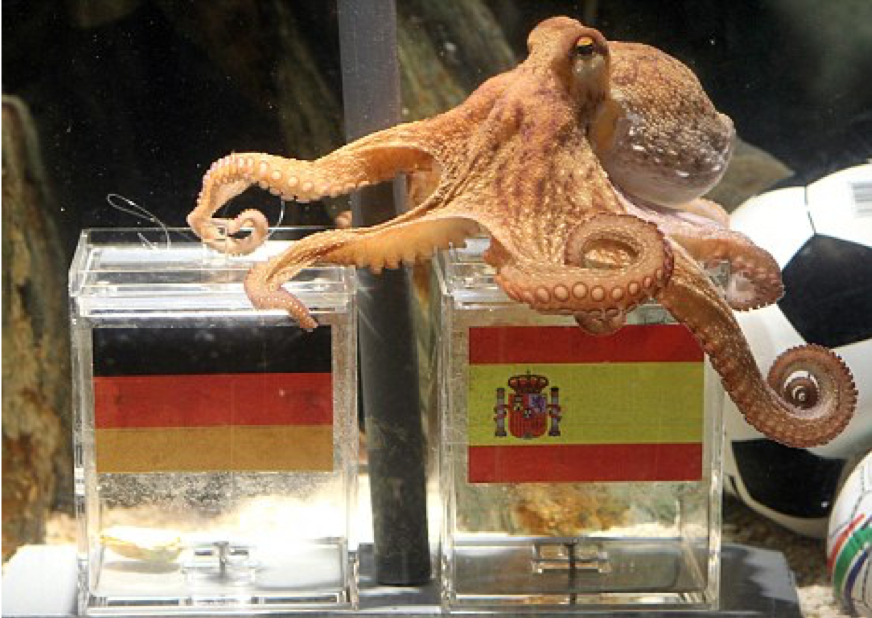
\includegraphics[width=0.4\tw]{20/fig-paul.png}

\end{multicols}

\bb
\ii What would this proportion be if Paul does not have psychic powers? If he does? Set up the null and alternative hypotheses in terms of the proportion of all correct guesses an octopus makes. Use appropriate notation. \vspace{1in}
\ii  How unusual would this be if Paul was just randomly guessing? Compute the P-value.   \vfill
\ii If a 5\% significance level is chosen, what is the result?   \vspace{1.5in}
\ee

\clearpage

\ii SAT math scores in the US in 2017 were normally distributed with a mean of 570 and a standard deviation of 107\footnote{\href{https://nces.ed.gov/programs/digest/d17/tables/dt17\_226.40.asp}{\underline{https://nces.ed.gov/programs/digest/d17/tables/dt17\_226.40.asp}}}. A high school district boasts their students are bright and their students are so good at math they can prove it (using a hypothesis test). A random sample of 25 seniors are selected, and the mean SAT math score of the sample is 613.
\bb
\ii Set up the null and alternative hypotheses both in words and using appropriate notation. \vspace{1in}
\ii  Compute the test statistic and interpret the meaning in practical terms. \vfill
\ii  Compute the P-value and interpret the meaning in practical terms. \vfill
\ii If a 5\% significance level is chosen, what is the result? If a 1\% significance level is chosen, what is the result?  \vspace{1.5in}
\ee


\clearpage

\ii Are we getting enough sleep?  It is generally recommended that adults sleep 8 hours per night. A random sample of 22  students at CU Denver had an average of $7.5$ hours with a standard deviation of $1.7$ hours. Is this evidence that sleeping patterns of students at CU Denver are different from the recommended amount of sleep?

\bb
\ii Set up the null and alternative hypotheses both in words and using appropriate notation. \vspace{1in}
\ii  Compute the test statistic and interpret the meaning in practical terms. \vfill
\ii  Compute the P-value and interpret the meaning in practical terms. \vfill
\ii If a 5\% significance level is chosen, what is the result? \vspace{1.5in}
\ee
\ee


\bbox
\bi
\ii Let $X_1, X_2, \ldots , X_n$  be a random sample from a normal population with unknown mean and standard deviation.  Let $\mu_0$ denote the value of $\mu$ claimed in $H_0$, then
\[ t = \frac{\bar{x}-\mu_0}{s/\sqrt{n}}.\]
We use a $t$-distribution with $n-1$ degrees of freedom to compute the corresponding P-value.
\ii Let $X$ be a binomial random and let $p_0$ denote the value of $p$ claimed in $H_0$.  If we observe $X=x$ successes out of $n$ trials, then we can find the P-value using a binomial distribution using the assumed probability of success, $p_0$.
\ei
\ebox

%\ii \textbf{Be nice to pigeons?} In a study\footnote{Belguermi, A., ``Pigeons discriminate between human feeders,'' \textit{Animal Cognition}, 2011} conducted in Paris, equal amounts of pigeon feed were spread on the ground in two adjacent locations. One person was assigned to be ``hostile'' and the other person ``nice''.  The two people were randomly exchanged between the two locations throughout the study. It seemed that the pigeons learned to avoid the hostile person's location.
